\documentclass[../main.tex]{subfiles}
\ifSubfilesClassLoaded{\setcounter{chapter}{12}}{}
\begin{document}

\chapter{Cross-Validation dan GridSearchCV Sederhana}

\begin{subcpmk}
  \item \textbf{Sub-CPMK-P9:} \texttt{cross\_val\_score} atau \texttt{cross\_validate}; \texttt{GridSearchCV} pada pipeline; test set tidak ikut tuning (RPS Mg.\ 12).
\end{subcpmk}

\SesiRPS{12}{P9}{$\sim$170 menit}{CPMK-P4}

\noindent Satu pemisahan latih/uji saja bisa beruntung atau sial karena sampel kecil. Validasi silang memberi estimasi kinerja dengan mencoba beberapa partisi; \texttt{GridSearchCV} menyisipkan pencarian hiperparameter di dalam lipatan tersebut---dengan catatan ketat bahwa \textbf{test set} tidak boleh dipakai untuk memilih model.

\section{Kemampuan akhir sesi}

Menjalankan CV untuk estimasi metrik; menyusun \texttt{GridSearchCV} pada \texttt{Pipeline}; menjelaskan mengapa evaluasi akhir pada \texttt{X\_test} hanya dilakukan sekali setelah tuning.

Tanpa disiplin ini, metrik uji menjadi optimistik: model secara tidak langsung ``melihat'' data uji melalui banyak percobaan hiperparameter. Dokumentasikan ruang pencarian yang dicoba agar hasil dapat diaudit.

\section{Teori}

\begin{konsep}
Validasi silang mengestimasi kinerja dengan rotasi partisi latih. \texttt{GridSearchCV} mencoba kombinasi hiperparameter pada ruang yang Anda tentukan. \textbf{Test set} hanya untuk laporan akhir setelah memilih model.
\end{konsep}

\texttt{Pipeline} di dalam CV memastikan setiap lipatan melakukan \texttt{fit\_transform} hanya pada data latih lipatan tersebut---konsisten dengan prinsip anti-leakage dari minggu prapemrosesan.

\begin{figure}[htbp]
\centering
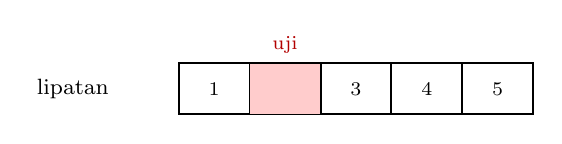
\begin{tikzpicture}[x=0.9cm,y=0.65cm]
  \foreach \f in {1,...,5} {
    \draw[thick] (\f,0) rectangle ++(1,1);
    \node[font=\scriptsize] at (\f+0.5,0.5) {\f};
  }
  \node[font=\footnotesize, anchor=east] at (0.15,0.5) {lipatan};
  \draw[fill=red!20] (2,0) rectangle ++(1,1);
  \node[font=\scriptsize, red!70!black] at (2.5,1.35) {uji};
\end{tikzpicture}
\caption{Skema validasi silang $k$-lipat ($k=5$): setiap lipatan bergantian menjadi partisi uji; skor dirata-rata untuk estimasi kinerja lebih stabil daripada satu split tunggal.}
\end{figure}


\begin{table}[htbp]
\centering
\caption{Peran partisi data saat tuning (ringkas).}
\label{tab:partisi-tuning}
\begin{tabular}{@{}p{3.2cm}p{9.5cm}@{}}
\toprule
\textbf{Subset} & \textbf{Fungsi} \\
\midrule
Train (dalam CV) & Latih model + pilih hiperparameter per lipatan. \\
Validation (implisit CV) & Estimasi kinerja sementara. \\
Test (hold-out) & Laporan akhir sekali, setelah model terpilih. \\
\bottomrule
\end{tabular}
\end{table}

\section{Contoh kode}

\noindent\textbf{cross\_val\_score.}
\begin{verbatim}
from sklearn.model_selection import cross_val_score
from sklearn.linear_model import LogisticRegression
from sklearn.datasets import load_iris

iris = load_iris()
X, y = iris.data, iris.target
clf = LogisticRegression(max_iter=300)
scores = cross_val_score(clf, X, y, cv=5)
print("CV akurasi", scores, "mean", scores.mean())
\end{verbatim}

\begin{verbatim}
from sklearn.pipeline import Pipeline
from sklearn.preprocessing import StandardScaler
from sklearn.model_selection import GridSearchCV, train_test_split
from sklearn.linear_model import LogisticRegression

X_train, X_test, y_train, y_test = train_test_split(
    X, y, test_size=0.2, random_state=42, stratify=y
)
pipe = Pipeline([
    ("sc", StandardScaler()),
    ("clf", LogisticRegression(max_iter=500)),
])
grid = {"clf__C": [0.1, 1.0, 10.0]}
search = GridSearchCV(pipe, grid, cv=5)
search.fit(X_train, y_train)
print("best params", search.best_params_)
print("test score", search.score(X_test, y_test))
\end{verbatim}

\begin{verbatim}
from sklearn.model_selection import cross_validate
import numpy as np
out = cross_validate(clf, X, y, cv=5, scoring=["accuracy", "f1_macro"])
print(np.mean(out["test_accuracy"]), np.mean(out["test_f1_macro"]))
\end{verbatim}

\noindent\textit{Checklist di Markdown notebook:} hiperparameter dipilih dari hasil CV pada data latih (bukan dari test); \texttt{X\_test} hanya untuk evaluasi akhir sekali.

\section{Referensi}

\begin{itemize}[leftmargin=*]
  \item Cross-validation. \url{https://scikit-learn.org/stable/modules/cross_validation.html}
  \item Grid search. \url{https://scikit-learn.org/stable/modules/grid_search.html}
\end{itemize}

\begin{asesmen}
\textbf{Tugas modul:} satu GridSearchCV dengan ruang parameter kecil + laporan skor test yang jujur.
\end{asesmen}

\begin{rangkuman}
Minggu 12 menstabilkan estimasi kinerja dan tuning terkendali.

\textbf{Kata kunci:} cross\_val\_score, GridSearchCV, Pipeline
\end{rangkuman}

\end{document}
